\chapter*{Практика 8. Расчет характеристик и построение графиков}
\addcontentsline{toc}{chapter}{Практика 8. Расчет характеристик и построение графиков}
\label{ch:8_practice}

\textit{\textbf{Задание:}} Провести анализ работы системы связи.

\begin{itemize}
    \item Проведено моделирование системы при различных параметрах:
    \begin{itemize}
        \item Различные отношения сигнал/шум
        \item Различное число лучей в канале
        \item Различные параметры модуляции
    \end{itemize}
    \item Построены графики зависимостей качества приёма от параметров системы
\end{itemize}

\begin{figure}[ht]
    \centering
    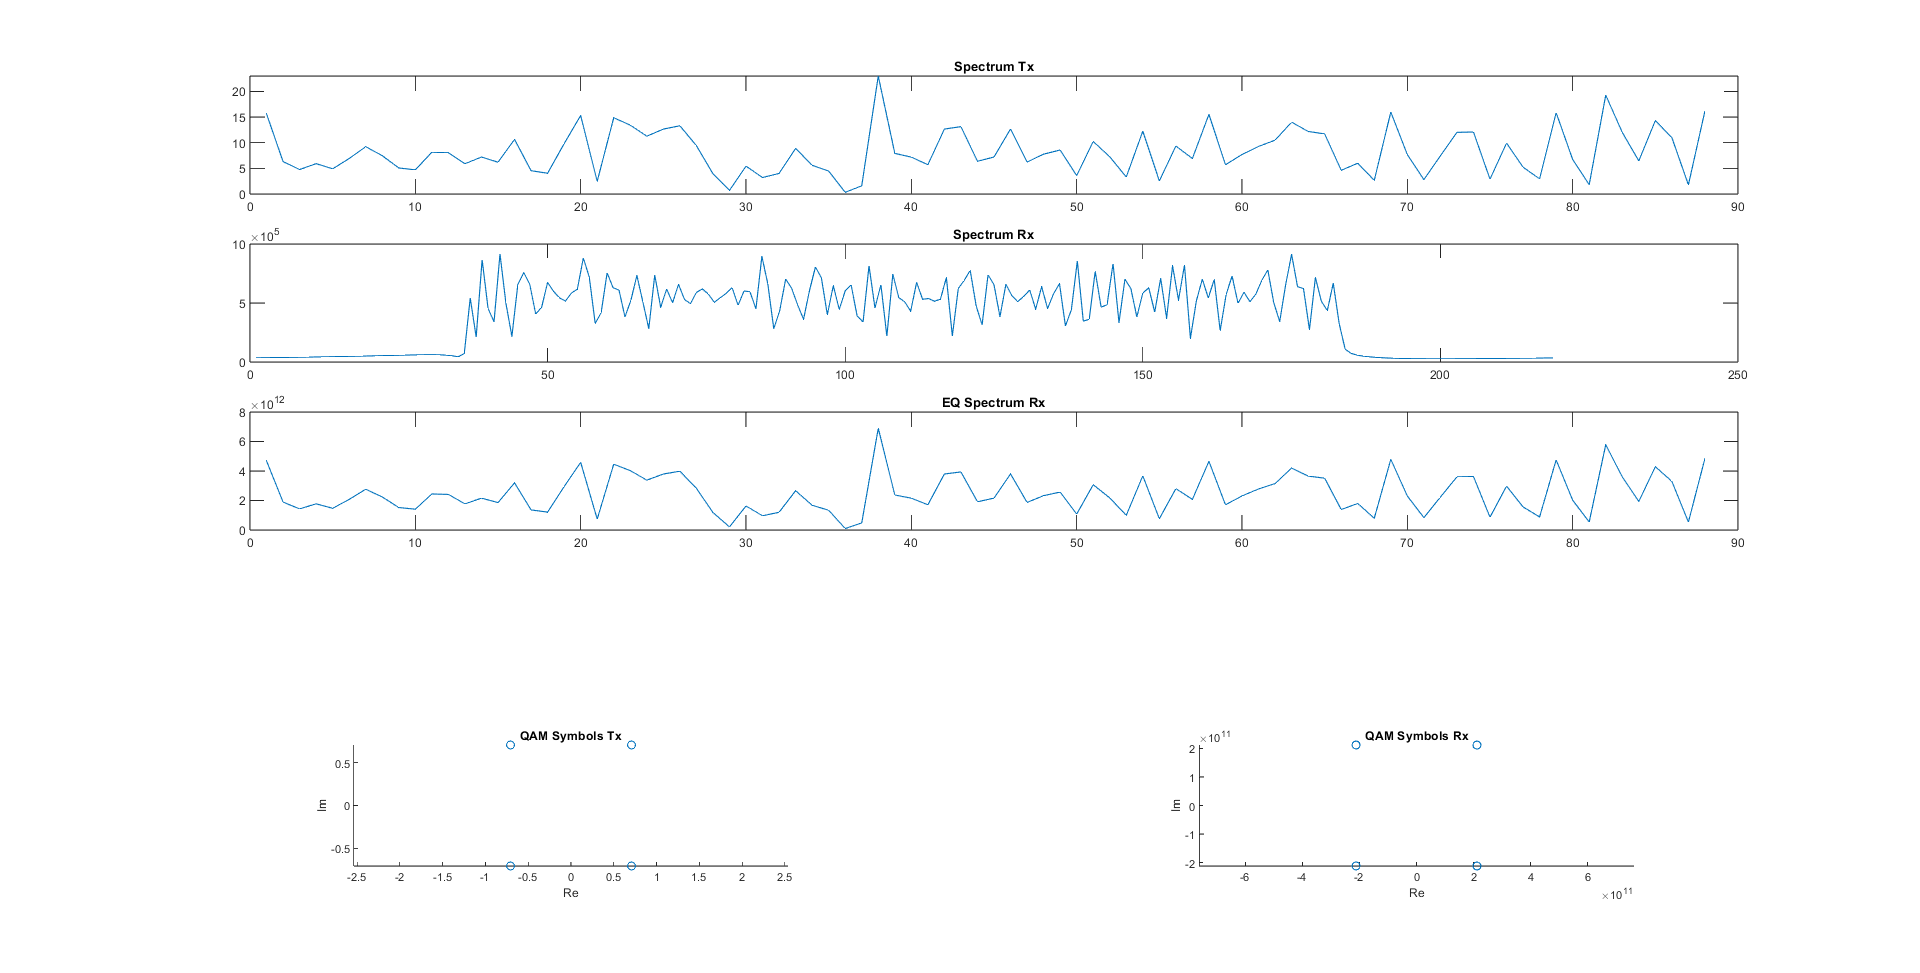
\includegraphics[width=0.8\textwidth]{8practice_result.png}
    \caption{Результат восьмой практики}
    \label{fig:8practice_result}
\end{figure}
